\begin{tomtat}
	\begin{minipage}[t]{0.3\textwidth}
		\vspace{0pt}
		\begin{tomtat}
			\begin{center}
				\textbf{ĐỀ 20}
			\end{center}
			
		\end{tomtat}
	\end{minipage}
	\hfill
	\begin{minipage}[t]{0.5\textwidth}
		\vspace{0pt}
		\begin{tomtat}
			\begin{center}
				\includegraphics[scale=0.08]{images/20}
			\end{center}
		\end{tomtat}
	\end{minipage}
\end{tomtat}
\textbf{I. PHẦN TRẮC NGHIỆM}
\begin{ex}
	Nghiệm của bất phương trình $-3x - 6 \ge 0$ là:
	\choice{$x \ge -2$}{$x \ge 2$}{$x \le 2$}{$x \le -2$}
	\loigiai{
		Ta có:
		$-3x - 6 \ge 0$
		$\Leftrightarrow -3x \ge 6$
		$\Leftrightarrow x \le \frac{6}{-3}$
		$\Leftrightarrow x \le -2$.
		\\ \textbf{Đáp Án D}
	}
\end{ex}

\begin{ex}
	Tìm giá trị của $x$ thoả mãn $x^3 = 3$ là:
	\choice{$3$}{$\sqrt[3]{3}$}{$-\sqrt[3]{3}$}{$-3$}
	\loigiai{
		Ta có: $x^3 = 3 \Leftrightarrow x = \sqrt[3]{3}$.
		\\ \textbf{Đáp Án B}
	}
\end{ex}

\begin{ex}
	Điểm nào sau đây thuộc hàm số $y = x^2$?
	\choice{$(-1; 2)$}{$(1; 2)$}{$(1; 1)$}{$(-2; 2)$}
	\loigiai{
		Xét các điểm:
		A. Với $(-1; 2)$: $y = (-1)^2 = 1 \neq 2$. Loại.
		B. Với $(1; 2)$: $y = 1^2 = 1 \neq 2$. Loại.
		C. Với $(1; 1)$: $y = 1^2 = 1$. Chọn.
		D. Với $(-2; 2)$: $y = (-2)^2 = 4 \neq 2$. Loại.
		Vậy điểm $(1;1)$ thuộc hàm số $y=x^2$.
		\\ \textbf{Đáp Án C}
	}
\end{ex}

\begin{ex}
	Cho tam giác ABC có $BC = 5$; $AC = 4$; $AB = 3$. Kết quả nào sau đây là đúng?
	\choice{$\sin C = 0,75$}{$\sin C = 0,8$}{$\sin C = 0,6$}{$\sin C = 1,3$}
	\loigiai{
		Ta thấy $AB^2 + AC^2 = 3^2 + 4^2 = 9 + 16 = 25$.
		$BC^2 = 5^2 = 25$.
		Do $AB^2 + AC^2 = BC^2$, nên tam giác ABC vuông tại A (theo định lý Pitago đảo).
		Trong tam giác ABC vuông tại A:
		$\sin C = \frac{\text{cạnh đối}}{\text{cạnh huyền}} = \frac{AB}{BC} = \frac{3}{5} = 0,6$.
		\\ \textbf{Đáp Án C}
	}
\end{ex}

\begin{ex}
	Góc nội tiếp chắn nửa đường tròn bằng bao nhiêu độ?
	\choice{$45^\circ$}{$90^\circ$}{$60^\circ$}{$120^\circ$}
	\loigiai{
		Theo định lý, góc nội tiếp chắn nửa đường tròn là góc vuông, có số đo bằng $90^\circ$.
		\\ \textbf{Đáp Án B}
	}
\end{ex}

\begin{ex}
	Khi tứ giác MNPQ nội tiếp đường tròn, và có góc M bằng $90^\circ$. Khi đó, góc P bằng:
	\choice{$100^\circ$}{$110^\circ$}{$180^\circ$}{$90^\circ$}
	\loigiai{
		Trong một tứ giác nội tiếp, tổng hai góc đối diện bằng $180^\circ$.
		Do đó, $\widehat{M} + \widehat{P} = 180^\circ$.
		Thay $\widehat{M} = 90^\circ$, ta có:
		$90^\circ + \widehat{P} = 180^\circ$
		$\widehat{P} = 180^\circ - 90^\circ = 90^\circ$.
		\\ \textbf{Đáp Án D}
	}
\end{ex}

\begin{ex}
	Cho hình trụ có bán kính đáy $R = 8$ cm và diện tích toàn phần $564\pi$ cm$^2$. Tính chiều cao của hình trụ.
	\choice{$27$ cm}{$27,25$ cm}{$25$ cm}{$25,27$ cm}
	\loigiai{
		Diện tích toàn phần của hình trụ được tính bằng công thức: $S_{tp} = 2\pi Rh + 2\pi R^2$.
		Theo đề bài, $R = 8$ cm và $S_{tp} = 564\pi$ cm$^2$.
		Ta có: $564\pi = 2\pi \cdot 8 \cdot h + 2\pi \cdot 8^2$
		$564\pi = 16\pi h + 128\pi$
		Chia cả hai vế cho $\pi$:
		$564 = 16h + 128$
		$16h = 564 - 128$
		$16h = 436$
		$h = \frac{436}{16} = \frac{109}{4} = 27,25$ cm.
		\\ \textbf{Đáp Án B}
	}
\end{ex}

\begin{ex}
	Cho đường tròn (O; 10cm), đường kính AB. Điểm M $\in$ (O) sao cho $\widehat{BAM} = 45^\circ$. Diện tích hình quạt AOM là:
	\choice{$5\pi \text{ (cm}^2\text{)}$}{$25\pi \text{ (cm}^2\text{)}$}{$50\pi \text{ (cm}^2\text{)}$}{$\frac{25}{2}\pi \text{ (cm}^2\text{)}$}
	\loigiai{
		Tam giác AOM có OA = OM = R = 10cm (bán kính).
		Do đó, tam giác AOM cân tại O.
		Ta có $\widehat{BAM} = \widehat{OAM} = 45^\circ$.
		Vì tam giác AOM cân tại O, nên $\widehat{OMA} = \widehat{OAM} = 45^\circ$.
		Số đo góc ở tâm $\widehat{AOM} = 180^\circ - (\widehat{OAM} + \widehat{OMA}) = 180^\circ - (45^\circ + 45^\circ) = 180^\circ - 90^\circ = 90^\circ$.
		Diện tích hình quạt tròn AOM được tính bằng công thức: $S_{qAOM} = \frac{\pi R^2 n}{360}$, với $n$ là số đo góc ở tâm.
		$S_{qAOM} = \frac{\pi \cdot 10^2 \cdot 90}{360} = \frac{100\pi \cdot 90}{360} = \frac{100\pi}{4} = 25\pi \text{ (cm}^2\text{)}$.
		\\ \textbf{Đáp Án B}
	}
\end{ex}

\newpage
\textbf{II. PHẦN TỰ LUẬN}
\begin{ex}
	Rút gọn: $P = \left( \frac{\sqrt{a}+2}{\sqrt{a}+1} - \frac{\sqrt{a}-2}{\sqrt{a}-1} \right) : \frac{1}{\sqrt{a}+1}$
	\loigiai{
		Điều kiện: $a \ge 0, a \neq 1$.
		Ta có:
		\begin{align*} P &= \left( \frac{(\sqrt{a}+2)(\sqrt{a}-1)}{(\sqrt{a}+1)(\sqrt{a}-1)} - \frac{(\sqrt{a}-2)(\sqrt{a}+1)}{(\sqrt{a}-1)(\sqrt{a}+1)} \right) \cdot (\sqrt{a}+1) \\ &= \frac{(a - \sqrt{a} + 2\sqrt{a} - 2) - (a + \sqrt{a} - 2\sqrt{a} - 2)}{(\sqrt{a}+1)(\sqrt{a}-1)} \cdot (\sqrt{a}+1) \\ &= \frac{(a + \sqrt{a} - 2) - (a - \sqrt{a} - 2)}{a-1} \cdot (\sqrt{a}+1) \\ &= \frac{a + \sqrt{a} - 2 - a + \sqrt{a} + 2}{a-1} \cdot (\sqrt{a}+1) \\ &= \frac{2\sqrt{a}}{(\sqrt{a}-1)(\sqrt{a}+1)} \cdot (\sqrt{a}+1) \\ &= \frac{2\sqrt{a}}{\sqrt{a}-1}\end{align*}
		Vậy $P = \frac{2\sqrt{a}}{\sqrt{a}-1}$.
	}
\end{ex}

\begin{ex}
	Giải hệ phương trình sau:
	$$ \begin{cases} x+2y=3 \\ x+y=2 \end{cases} $$
	\loigiai{
		Ta có hệ phương trình:
		$$ \begin{cases} x+2y=3 \quad &(1) \\ x+y=2 \quad &(2) \end{cases} $$
		Trừ vế theo vế của phương trình (1) cho phương trình (2), ta được:
		$(x+2y) - (x+y) = 3 - 2$
		$y = 1$.
		Thay $y=1$ vào phương trình (2):
		$x + 1 = 2$
		$x = 1$.
		Vậy nghiệm của hệ phương trình là $(x; y) = (1; 1)$.
	}
\end{ex}

\begin{ex}
	Cho phương trình $x^2+3x-1=0$. Gọi $x_1, x_2$ là hai nghiệm của phương trình. Tính giá trị của biểu thức: $A=2x_1^2x_2^2-4x_1^2-4x_2^2$.
	\loigiai{
		Phương trình $x^2+3x-1=0$ có $a=1, b=3, c=-1$.
		Vì $ac = 1 \cdot (-1) = -1 < 0$, phương trình luôn có hai nghiệm phân biệt $x_1, x_2$.
		Theo hệ thức Vi-ét, ta có:
		$$ \begin{cases} x_1 + x_2 = -\frac{b}{a} = -\frac{3}{1} = -3 \\ x_1 x_2 = \frac{c}{a} = \frac{-1}{1} = -1 \end{cases} $$
		Ta biến đổi biểu thức A:
		\begin{align*} A &= 2x_1^2x_2^2 - 4x_1^2 - 4x_2^2 \\ &= 2(x_1x_2)^2 - 4(x_1^2 + x_2^2) \\ &= 2(x_1x_2)^2 - 4((x_1+x_2)^2 - 2x_1x_2)\end{align*}
		Thay giá trị từ hệ thức Vi-ét vào biểu thức A:
		\begin{align*} A &= 2(-1)^2 - 4((-3)^2 - 2(-1)) \\ &= 2(1) - 4(9 + 2) \\ &= 2 - 4(11) \\ &= 2 - 44 \\ &= -42\end{align*}
		Vậy $A = -42$.
	}
\end{ex}

\begin{ex}
	Một xí nghiệp sản xuất được 120 sản phẩm loại I và 120 sản phẩm loại II trong thời gian 7h. Mỗi giờ sản xuất được số sản phẩm loại I ít hơn số sản phẩm loại II là 10 sản phẩm. Hỏi mỗi giờ xí nghiệp sản xuất được bao nhiêu sản phẩm mỗi loại?
	\loigiai{
		Gọi số sản phẩm loại I xí nghiệp sản xuất được trong một giờ là $x$ (sản phẩm, $x > 0$).
		Khi đó, số sản phẩm loại II xí nghiệp sản xuất được trong một giờ là $x+10$ (sản phẩm).
		
		Thời gian để sản xuất 120 sản phẩm loại I là: $\frac{120}{x}$ (giờ).
		Thời gian để sản xuất 120 sản phẩm loại II là: $\frac{120}{x+10}$ (giờ).
		
		Tổng thời gian sản xuất cả hai loại sản phẩm là 7 giờ, nên ta có phương trình:
		$\frac{120}{x} + \frac{120}{x+10} = 7$
		Điều kiện: $x > 0$.
		Quy đồng mẫu số và giải phương trình:
		\begin{align*}
			\frac{120(x+10) + 120x}{x(x+10)} &= 7 \\
			120(x+10) + 120x &= 7x(x+10) \\
			120x + 1200 + 120x &= 7x^2 + 70x \\
			240x + 1200 &= 7x^2 + 70x \\
			7x^2 + 70x - 240x - 1200 &= 0 \\
			7x^2 - 170x - 1200 &= 0
		\end{align*}
		Giải phương trình bậc hai $7x^2 - 170x - 1200 = 0$:
		Ta có $\Delta = b^2 - 4ac = (-170)^2 - 4(7)(-1200) = 28900 + 33600 = 62500$.
		$\sqrt{\Delta} = \sqrt{62500} = 250$.
		Phương trình có hai nghiệm phân biệt:
		$x_1 = \frac{-b + \sqrt{\Delta}}{2a} = \frac{170 + 250}{2 \cdot 7} = \frac{420}{14} = 30$.
		$x_2 = \frac{-b - \sqrt{\Delta}}{2a} = \frac{170 - 250}{2 \cdot 7} = \frac{-80}{14} = -\frac{40}{7}$.
		
		Vì $x > 0$, nên ta nhận $x = 30$.
		Vậy, số sản phẩm loại I sản xuất được trong một giờ là 30 sản phẩm.
		Số sản phẩm loại II sản xuất được trong một giờ là $x+10 = 30+10 = 40$ sản phẩm.
		
		Vậy, mỗi giờ xí nghiệp sản xuất được 30 sản phẩm loại I và 40 sản phẩm loại II.
	}
\end{ex}
\begin{ex}
	Một toà nhà chung cư có 30 tầng, được đánh số lần lượt từ 1 đến 30. Bạn Bình vào thang máy ở tầng 1, bấm chọn ngẫu nhiên số một tầng để đi lên. Tính xác suất của các biến cố A: “Bình đi lên tầng có số là một số nguyên tố”.
	\loigiai{
		Bạn Bình ở tầng 1 và bấm chọn ngẫu nhiên một tầng để đi lên, các tầng có thể đến là từ tầng 2 đến tầng 30.\\
		Không gian mẫu $\Omega = \{2; 3; 4; \dots; 29; 30\}$.\\
		Số phần tử của không gian mẫu là $n(\Omega) = 30 - 2 + 1 = 29$.\\
		Biến cố A: “Bình đi lên tầng có số là một số nguyên tố”.\\
		Các số nguyên tố trong các tầng Bình có thể đến (từ 2 đến 30) là:
		$A = \{2; 3; 5; 7; 11; 13; 17; 19; 23; 29\}$.\\
		Số phần tử của biến cố A là $n(A) = 10$.
		Xác suất của biến cố A là:
		$P(A) = \frac{n(A)}{n(\Omega)} = \frac{10}{29}$.
	}
\end{ex}
\begin{ex}
	Cho đường tròn (O;R) và dây cung AB < 2R. Gọi H là trung điểm của AB, đường thẳng HO cắt đường tròn (O) tại hai điểm C và D (C thuộc cung nhỏ AB). Điểm M thuộc đoạn AH (M khác A và H), tia CM cắt đường tròn (O) tại điểm thứ hai là N. Gọi I là giao điểm của hai đường thẳng DN và AB, K là giao điểm của hai đường thẳng CI và DM.
	\begin{enumerate}
		\item[a)] Chứng minh rằng: Bốn điểm I, A, M, N thuộc 1 đường tròn.
		\item[b)] Chứng minh rằng $CM \cdot CN = CK \cdot CI$ và M là tâm đường tròn nội tiếp tam giác HKN.
	\end{enumerate}
	\loigiai{
	\begin{center}
		
		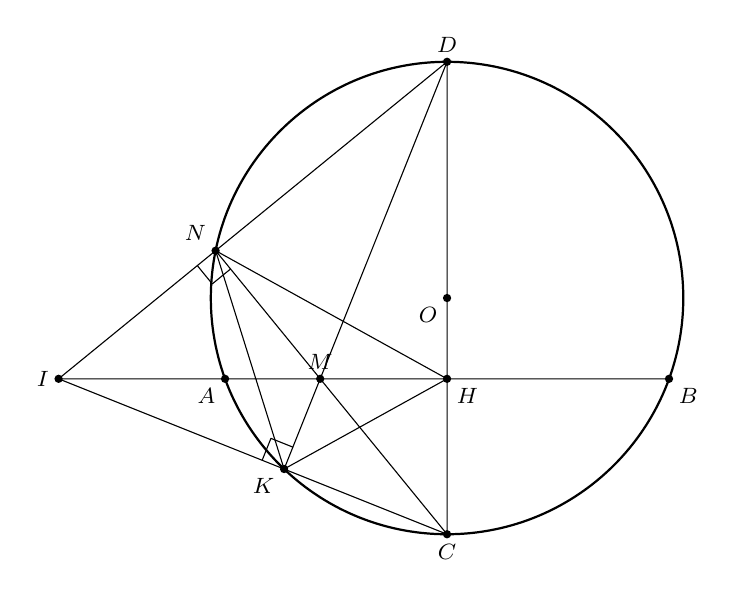
\begin{tikzpicture}[line join = round, line cap=round,>=stealth,font=\footnotesize,scale=1]
			\usetikzlibrary{calc,intersections,angles} % Added intersections
			% Def
			\def\r{3}
			
			% Coordinates
			\coordinate (O) at (0,0);
			\coordinate (D) at (90:\r);    % D on positive y-axis
			\coordinate (A) at (-160:\r);  % A in Q3
			\coordinate (B) at (-20:\r);   % B in Q4
			\coordinate (C) at (-90:\r);   % C on negative y-axis
			
			% H is midpoint of AB
			\coordinate (H) at ($ (A)!0.5!(B) $);
			
			% I such that vector IA = 3/8 vector AB
			% vec(I) = vec(A) - 3/8 * (vec(B) - vec(A)) = 11/8*vec(A) - 3/8*vec(B)
			\coordinate (I) at ($ 11/8*(A) - 3/8*(B) $);
			
			% N is projection of C onto ID
			\coordinate (N) at ($ (I)!(C)!(D) $);
			
			% K is projection of D onto IC
			\coordinate (K) at ($ (I)!(D)!(C) $);
			
			% M is intersection of DK and NC
			% Define paths for intersection
			\path[name path=DKline] (D) -- (K);
			\path[name path=NCline] (N) -- (C);
			% Find intersection
			\path[name intersections={of=DKline and NCline, by=M}];
			
			% Draw
			% Draw circle (O,r)
			\draw[thick] (O) circle (\r);
			
			% Draw paths I-D-C-I (triangle IDC)
			\draw (I) -- (D) -- (C) -- cycle; 
			
			% Draw path I-B-H-N-K-H
			\draw (I) -- (B) -- (H) -- (N) -- (K) -- (H);
			
			% Draw N-C
			\draw (N) -- (C);
			
			% Draw D-K
			\draw (D) -- (K);
			
			% Fill points
			\fill (O) circle (1.5pt);
			\fill (D) circle (1.5pt);
			\fill (A) circle (1.5pt);
			\fill (B) circle (1.5pt);
			\fill (C) circle (1.5pt);
			\fill (H) circle (1.5pt);
			\fill (I) circle (1.5pt);
			\fill (N) circle (1.5pt);
			\fill (K) circle (1.5pt);
			\fill (M) circle (1.5pt);
			
			% Node points (old style)
			\node[below left] at (O) {$O$};
			\node[above] at (D) {$D$};       % D is (0,3)
			\node[below left] at (A) {$A$};  % A is approx (-2.8, -1.0)
			\node[below right] at (B) {$B$}; % B is approx (2.8, -1.0)
			\node[below] at (C) {$C$};       % C is (0,-3)
			\node[below right] at (H) {$H$};       % H is approx (0, -1.0)
			\node[left] at (I) {$I$};         % I is approx (-4.9, -1.0)
			\node[above left] at (N) {$N$}; % N is on ID, depends on projection
			\node[below left] at (K) {$K$};  % K is on IC, depends on projection
			\node[above] at (M) {$M$};       % M is intersection, position varies
			
			% Ky hieu goc vuong (old style)
			% CN is perpendicular to ID
			\pic[draw, angle radius=3mm]{right angle = C--N--I}; % or C--N--D
			% DK is perpendicular to IC
			\pic[draw, angle radius=3mm]{right angle = D--K--I}; % or D--K--C
			
			\end{tikzpicture}
				
	\end{center}
	
	}
\end{ex}

\begin{ex}
	Một trường THCS làm sân chơi thể thao, mặt sân có dạng hình chữ nhật với chiều dài hơn chiều rộng 7 mét. Số tiền làm mặt sân là 62\,400\,000 đồng. Biết rằng chi phí làm mỗi mét vuông mặt sân là 800\,000 đồng. Tính chiều dài và chiều rộng của mặt sân.
\end{ex}

\begin{ex}
	Cho 3 số dương a, b, c thỏa mãn $abc = 1$. Chứng minh:
	$$ \frac{1}{a^3 + b^3 + 1} + \frac{1}{b^3 + c^3 + 1} + \frac{1}{c^3 + a^3 + 1} \le 1 $$
	(Lưu ý: Trong đề bài gốc của bạn, mẫu số đầu tiên là $x^3 + b^3 + 1$. Tôi giả định đó là một lỗi nhỏ và đã sửa thành $a^3 + b^3 + 1$ để phù hợp với tính đối xứng của bài toán. Nếu $x$ là một biến khác, bạn vui lòng cho biết.)
\end{ex}


\setcounterref{ex}{0}
